\documentclass{uimppracticas}

%Permitir cabeceras y pie de páginas personalizados
\pagestyle{fancy}

%Path por defecto de las imágenes
\graphicspath{ {./images/} }

%Declarar formato de encabezado y pie de página de las páginas del documento
\fancypagestyle{doc}{
	%Pie de Página
	\footerpr{}{}{{\thepage} de \pageref{LastPage}}
}

%Declarar formato de encabezado y pie del título e indice
\fancypagestyle{titu}{%
	%Cabecera
	\headerpr{}{}{}
	%Pie de Página
	\footerpr{}{}{}
}

\appto\frontmatter{\pagestyle{titu}}
\appto\mainmatter{\pagestyle{doc}}

\begin{document}
	
%Comienzo formato título
\frontmatter

%Portada (Centrado todo)
\centeredtitle{./images/LogoUIMP.png}{Máster Universitario en Investigación en Inteligencia Artificial}{Curso 2020-2021}{Sistemas de Recomendación}{Recomendación para grupos \\ en Python}

\begin{center}
	\large \today
\end{center}

\vspace{40mm}

\begin{flushright}
	{\bf Laura Rodríguez Navas}\\
	\textbf{DNI:} 43630508Z\\
	\textbf{e-mail:} \href{rodrigueznavas@posgrado.uimp.es}{rodrigueznavas@posgrado.uimp.es}
\end{flushright}

\newpage

%Índice
\tableofcontents

\newpage

%Comienzo formato documento general
\mainmatter

\setlength\parskip{2.5ex}

\section{Introducción}\label{introducción}

El crecimiento de Internet y de la información disponible en línea ha hecho que sea mucho más difícil extraer información útil de manera efectiva. La abrumadora cantidad de datos requiere de mecanismos de filtrado de información eficientes. Y uno de los sistemas utilizados para hacer frente a este problema son los sistemas de recomendación.

Los sistemas de recomendación pueden definirse como herramientas diseñadas para interactuar con conjuntos de información grandes y complejos con la finalidad de proporcionar al usuario información o elementos que sean de su interés, todo ello de forma automatizada. Su funcionamiento se basa en el empleo de métodos matemáticos y estadísticos capaces de explotar la información previamente almacenada y crear recomendaciones adaptadas a cada usuario. En la actualidad, los sistemas de recomendación son una tecnología implementada en la mayoría de plataformas online como \textit{Amazon}, \textit{Neflix}, \textit{Spotify}, etc; ya que han dado muy buenos resultados incrementando las ventas. Los sistemas de recomendación también están presentes en muchos otros ámbitos, como por ejemplo el de las noticias, mostrando al usuario noticias que le interesan. La mayoría de los sistemas de recomendación se pueden clasificar en tres grupos: \textbf{basados en contenido}, \textbf{filtrado colaborativo} y \textbf{híbridos} (combinación de los dos anteriores).

En este documento se describe el desarrollo práctico en Python de un sistema de recomendación. El sistema de recomendación elegido aplica la técnica de filtrado colaborativo (\textit{user-based}). La implementación se puede encontrar en~\cite{GitHubRepo}, la cual está formada por el desarrollo del programa que implementa un sistema de recomendación de \href{https://es.wikipedia.org/wiki/Filtrado_colaborativo}{filtrado colaborativo} basado en usuarios. 

El documento se divide en diferentes secciones donde se va describiendo paso a paso el trabajo realizado. En la primera parte del documento se describe la técnica de filtrado colaborativo elegida, con sus ventajas y desventajas (ver secciones~\ref{filtro_colaborativo} y~\ref{ventajas_desventajas}). El documento sigue con la descripción del conjunto de datos que usamos con el sistema de recomendación y cómo podemos adquirirlo (ver sección~\ref{conjunto_datos}).

En la sección~\ref{sistema_recomendacion} del documento se describe paso a paso la implementación en Python del sistema de recomendación de filtrado colaborativo basado en usuarios. En esta sección también se describe el \href{https://es.wikipedia.org/wiki/Coeficiente_de_correlaci\%C3\%B3n_de_Pearson}{coeficiente de Correlación de Pearson} y porqué se ha elegido como medida de similitud para encontrar las correlaciones entre las valoraciones de los usuarios representados por el conjunto de datos y un nuevo usuario que se añade para recomendarle elementos de su interés respecto a las valoraciones de los otros usuarios (ver sección~\ref{correlacion_pearson}). En la siguiente sección, la~\ref{resultados}, se presentan las recomendaciones que crea el sistema de recomendación para el nuevo usuario y finalmente, en la parte final del documento se añaden las conclusiones y la bibliografía.

\subsection{Filtrado Colaborativo}\label{filtro_colaborativo}

La técnica de filtrado colaborativo basada en usuarios (\textit{collaborative filtering user-based}) se fundamenta en la idea de \textit{muéstrame cosas que le hayan gustado a gente parecida a mí}. Para que este tipo de sistema de recomendación funcione se necesita disponer de las valoraciones de los usuarios para poder agruparlos por similitud. Sin embargo, no se necesita conocer la descripción detallada de los elementos que se quieren recomendar. La limitación de este tipo de sistema aparece en el momento en que se une un nuevo usuario, ya que, hasta que no se dispone de suficiente información sobre sus valoraciones, no se pueden hacer recomendaciones. Este problema se denomina el problema del \href{https://es.wikipedia.org/wiki/Arranque_en_fr\%C3\%ADo}{comienzo frío} (\textit{cold start}).

En esta práctica el Filtrado Colaborativo (FC) nos permitirá crear recomendaciones personalizadas a un nuevo usuario, encontrando elementos de su interés con el análisis de datos de otros usuarios; asumiendo que los usuarios con intereses parecidos tienden a hacer valoraciones de forma similar. Es decir, para predecir la valoración que un usuario \textit{A} hará de un elemento \textit{X} que todavía no ha visto, se buscan usuarios con intereses similares a \textit{A} y se utilizan las valoraciones de estos otros usuarios sobre el elemento \textit{X} como estimación de la valoración del usuario \textit{A}. En resumen, el filtrado colaborativo basado en usuarios es un método para hacer predicciones automáticas (filtrado) sobre los intereses de un usuario mediante la recopilación de las valoraciones de muchos usuarios (colaboradores). Estos sistemas usualmente siguen una metodología que puede reducirse en:

\begin{enumerate}
	\item La búsqueda de usuarios que comparten los mismos patrones de valoración con el usuario activo (el usuario para el que se está haciendo la predicción).
	\item Utilizar las valoraciones por parte de aquellos usuarios afines que se encuentran en el paso 1 al fin de calcular una predicción para el usuario activo.
\end{enumerate}

En la sección~\ref{sistema_recomendacion} se describe detalladamente la metodología desarrollada en Python del sistema de recomendación de filtrado colaborativo basado en usuarios.

\subsection{Ventajas y Desventajas del Filtrado Colaborativo}\label{ventajas_desventajas}

Los SR colaborativos tienen importantes ventajas respecto a los no colaborativos:

\begin{itemize}
	\item Dan un mayor soporte para el filtrado de elementos cuyo contenido no es fácil de analizar por procesos automatizados.
	\item Dan la posibilidad de filtrar elementos basándose en su calidad o preferencias.
	\item Se adaptan a los intereses del usuario si estos cambian con el tiempo.
	\item Realizan recomendaciones válidas, pero que no esperábamos, lo cual puede resultar de gran utilidad.
\end{itemize}

Sin embargo, también presentan inconvenientes:

\begin{itemize}
	\item Son difíciles de aplicar en grandes cantidades de usuarios.
	\item A veces no encuentran suficientes usuarios para realizar recomendaciones a un nuevo usuario, cuando el número de usuarios del conjunto de datos es bajo.
	\item No trabajan bien a la hora de filtrar información para necesidades de contenido específicas, o cuando tenemos pocos datos de un nuevo usuario. Este problema se ha comentado en la sección anterior, se denomina problema del comienzo frío.
\end{itemize}

Para aliviar los inconvenientes se suele recurrir a sistemas de recomendación híbridos, que utilizan a la vez sistemas de recomendación de filtrado colaborativo y sistemas de recomendación basados en contenido (\textit{content-based filtering}). Los sistemas de recomendación basados en contenido se fundamentan en la idea de \textit{muéstrame más cosas como las que me han gustado}. Es de esperar que, a partir de los elementos que han sido valorados positivamente por un usuario, se puedan recomendar a otros usuarios cuyas características se asemejen a los anteriores. 

En esta práctica no me ha parecido adecuado el desarrollo de un sistema de recomendación híbrido, porqué se me podría haber complicado el desarrollo en Python. Y al ser mi primera implementación en Python de un sistema de recomendación, mi decisión ha sido centrarme en un tipo de SR.

\section{Conjunto de datos}\label{conjunto_datos}

El conjunto de datos que se ha usado en esta práctica se encuentra disponible públicamente para su descarga en el siguiente enlace: \url{https://www.kaggle.com/abhikjha/movielens-100k/download}. Este conjunto de datos se llama \textit{ml-latest-small}, contiene valoraciones de películas con valores entre 1 y 5 estrellas, y la actividad del etiquetado de \href{http://movielens.org}{MovieLens}~\cite{MovieLens}, un servicio de recomendación de películas. Exactamente, el conjunto de datos contiene 100836 valoraciones y 3683 etiquetas de 9742 películas. Los datos fueron creados por 610 usuarios que se seleccionaron al azar. Cada usuario clasificó al menos 20 películas diferentes y está representado por un identificador.

Una vez descargado el conjunto de datos podemos ver que está contenido en los archivos \textit{links.csv}, \textit{movies.csv}, \textit{ratings.csv} y \textit{tags.csv}. Aunque para esta práctica solo se utilizan los archivos \textit{movies.csv} y \textit{ratings.csv}. Estos archivos se pueden encontrar en la carpeta \textit{dataset} y en la carpeta con el mismo nombre en el repositorio~\cite{GitHubRepo}.

Con la finalidad de mejorar las recomendaciones del sistema de recomendación, realizaremos un seguido de transformaciones en el conjunto de datos. Para empezar, cargamos los archivos \textit{movies.csv} y \textit{ratings.csv} dentro de un dataframe (ver Definición~\ref{dataframe}) con el uso de la librería pandas~\cite{pandas} de Python. Se ha decidido trabajar con esta librería porqué permite leer y escribir fácilmente ficheros en formato CSV, acceder a los datos mediante índices o nombres para filas y columnas, ofrece métodos para reordenar, dividir y combinar conjuntos de datos, etc. y todo ello de forma muy eficiente.

\begin{lstlisting}[language=python, basicstyle=\small]
movies_df = pd.read_csv('dataset/movies.csv')
ratings_df = pd.read_csv('dataset/ratings.csv')
\end{lstlisting}

Miramos el contenido de \textit{movies\_df} para ver cómo ha quedado organizado:

\begin{table}[H]
	\centering
	\begin{tabular}{cll}
		\toprule
		movieId &                         title &                                       genres \\
		\midrule
		1 &                    Toy Story (1995) &  Adventure|Animation|Children|Comedy|Fantasy \\
		2 &                      Jumanji (1995) &                   Adventure|Children|Fantasy \\
		3 &             Grumpier Old Men (1995) &                               Comedy|Romance \\
		4 &            Waiting to Exhale (1995) &                         Comedy|Drama|Romance \\
		5 &  Father of the Bride Part II (1995) &                                       Comedy \\
		6 &                         Heat (1995) &                        Action|Crime|Thriller \\
		7 &                      Sabrina (1995) &                               Comedy|Romance \\
		8 &                 Tom and Huck (1995) &                           Adventure|Children \\
		9 &                 Sudden Death (1995) &                                       Action \\
		10 &                    GoldenEye (1995) &                    Action|Adventure|Thriller \\
		\bottomrule
	\end{tabular}
	\caption{Contenido preliminar del dataframe \textit{movies\_df}.}
	\label{movies_df}
\end{table}

Observando la Tabla~\ref{movies_df}, vemos que cada película tiene un único identificador (\textit{movieId}), un título, su año de estreno y diferentes géneros. Como los años del estreno de las películas contienen caracteres \textit{unicode}, los sacaremos de la columna de los títulos y los ubicaremos en una nueva columna que nombraremos \textit{year}. Para ello, primero creamos una expresión regular con el fin de seleccionar los años guardados entre paréntesis, y con la función \textit{extract} de la librería pandas los extraemos para guardarlos en su propia columna. Después borramos los años en la columna de los títulos con la función \textit{replace}, y para acabar, con la función \textit{strip} nos aseguramos de sacar los espacios extra que pudieran haber quedado durante el proceso de transformación. Además, eliminamos la columna de los géneros con la función \textit{drop}, ya que no la tendremos en cuenta más adelante en el sistema de recomendación.

\newpage

\begin{lstlisting}[language=python, basicstyle=\small]
regular_expression = r'\((.*?)\)'
movies_df['year'] = movies_df.title.str.lower().str.extract(regular_expression)
movies_df['title'] = movies_df.title.str.replace(regular_expression, '', regex=True)
movies_df['title'] = movies_df['title'].apply(lambda x: x.strip())
movies_df = movies_df.drop('genres', 1)
\end{lstlisting}

Vemos el resultado:

\begin{table}[H]
	\centering
	\begin{tabular}{clc}
		\toprule
		movieId &                  title &  year \\
		\midrule
		1 &                    Toy Story &  1995 \\
		2 &                      Jumanji &  1995 \\
		3 &             Grumpier Old Men &  1995 \\
		4 &            Waiting to Exhale &  1995 \\
		5 &  Father of the Bride Part II &  1995 \\
		6 &                         Heat &  1995 \\
		7 &                      Sabrina &  1995 \\
		8 &                 Tom and Huck &  1995 \\
		9 &                 Sudden Death &  1995 \\
		10 &                    GoldenEye &  1995 \\
		\bottomrule
	\end{tabular}
	\caption{Contenido del dataframe \textit{movies\_df}.}
	\label{movies_df_final}
\end{table}

\begin{definition}\label{dataframe}
	Un DataFrame es una estructura de datos bidimensional y etiquetada que acepta diferentes tipos datos de entrada organizados en columnas. Se puede pensar en un DataFrame como una hoja de cálculo o una tabla SQL.
\end{definition}

Ahora, miramos el contenido de \textit{ratings\_df} para ver cómo ha quedado organizado. Pero antes, eliminamos la columna \textit{timestamp}, porqué tampoco la tendremos en cuenta más adelante en el sistema de recomendación.

\begin{lstlisting}[language=python, basicstyle=\small]
ratings_df = ratings_df.drop('timestamp', 1)
\end{lstlisting}

Así queda organizado el contenido en \textit{ratings\_df}:

\begin{table}[H]
	\centering
	\begin{tabular}{ccc}
		\toprule
		userId &  movieId &  rating \\
		\midrule
		1 &        1 &     4.0 \\
		1 &        3 &     4.0 \\
		1 &        6 &     4.0 \\
		1 &       47 &     5.0 \\
		1 &       50 &     5.0 \\
		1 &       70 &     3.0 \\
		1 &      101 &     5.0 \\
		1 &      110 &     4.0 \\
		1 &      151 &     5.0 \\
		1 &      157 &     5.0 \\
		\bottomrule
	\end{tabular}
	\caption{Contenido del dataframe \textit{ratings\_df}.}
	\label{ratings_df}
\end{table}

Observando la Tabla~\ref{ratings_df}, vemos que cada fila del dataframe \textit{ratings\_df} contiene un identificador de usuario (asociado con al menos una película) y la valoración que este ha realizado de cada una de ellas. Por ejemplo, vemos que el usuario 1 ha visto y valorado diferentes películas (1, 3, 6, 47, 50, etc.).

\section{Sistema de Recomendación}\label{sistema_recomendacion}

En esta sección describimos detalladamente el sistema de recomendación desarrollado en Python~\cite{GitHubRepo}, que como se ha comentado en la sección~\ref{filtro_colaborativo}, utiliza la técnica de filtrado colaborativo basado en usuarios. Con esta técnica entrenaremos al sistema para predecir recomendaciones de películas a un nuevo usuario acordes a sus intereses. Para predecir estas recomendaciones, el sistema de recomendación buscará las similitudes entre las valoraciones introducidas por el nuevo usuario con las valoraciones de los otros usuarios ya existentes en el sistema. Es decir, el sistema de recomendación intentará encontrar usuarios que tengan valoraciones parecidas a las del nuevo usuario y entonces recomendarle películas acordes a sus valoraciones. 

A la hora de entrenar el sistema de recomendación, es crítico entender de qué forma se están haciendo las valoraciones, porqué dependiendo de ello, se pueden emplear varios métodos para definir y cuantificar la similitud entre los usuarios. En este caso, según el conjunto de datos anteriormente visto en la sección~\ref{conjunto_datos}, las valoraciones son numéricas, es decir, las valoraciones se hacen empleando una escala numérica de 1 a 5 estrellas. Y personalmente el método que me pareció más adecuado para calcular la similitud entre los usuarios de este conjunto de datos fue un método que se basa en \href{https://es.wikipedia.org/wiki/Coeficiente_de_correlaci\%C3\%B3n_de_Pearson}{correlación Pearson} (ver sección~\ref{correlacion_pearson}). También porqué es uno de los métodos que más he utilizado con anterioridad a la realización de esta práctica.

El objetivo de este sistema de recomendación es recomendar 10 películas a un nuevo usuario, mediante la estrategia siguiente:

\begin{enumerate}
	\item Crear un nuevo usuario identificando algunas de las películas del conjunto de datos que haya visto. Se asume que estas películas serán valoradas por el nuevo usuario.
	\item Basándose en la selección de las películas vistas por el nuevo usuario, obtener las películas donde el nuevo usuario y los otros usuarios coinciden, es decir, encontrar las películas que tanto el nuevo usuario como sus vecinos (usuarios similares a él) hayan visto.
	\item Calcular la similitud entre el nuevo usuario y sus vecinos en base a sus perfiles de valoración, es decir, utilizando los vectores formados por sus valoraciones. Se emplea la correlación de Pearson como medida de similitud.
	\item Para cada una de las películas obtenidas en el paso 2:
		\begin{itemize}
			\item Seleccionar los K=50 usuarios más parecidos al nuevo usuario (selección de vecindario), cuyo valor de similitud es positivo. En la práctica, el número óptimo de usuarios debería identificarse mediante validación cruzada, sin embargo, para no añadir una capa de complejidad extra a la práctica, he decidido emplear este valor.
			\item Calcular la media ponderada de las valoraciones que los K=50 usuarios han dado a la película. Este valor se almacena como el valor predicho de la película.
		\end{itemize}	
	\item Mostrar como recomendaciones las 10 películas con mayor valor predicho.
\end{enumerate}

Afín de seguir la estrategia anterior, comenzamos creando un nuevo usuario a quien recomendar películas. Para ello, hemos creado el archivo \textit{new\_user.csv} dentro de la carpeta \textit{dataset}, y le hemos añadido los títulos de 100 películas elegidas aleatoriamente del conjunto de datos con una nueva valoración, que, en este caso, he valorado según mi criterio. El archivo textit{new\_user.csv} se puede modificar como se desee para realizar tantas recomendaciones como se quiera, solo debemos asegurarnos de escribir bien los títulos de las películas, igual que aparecen en el archivo \textit{dataset/movies.csv}, y que valoramos las películas con un valor entre 1 y 5 estrellas. En la Figura~\ref{new_user}, podemos observar cómo se organiza parte del contenido del archivo \textit{new\_user.csv}, y que cargamos en un nuevo dataframe que nombramos \textit{user\_df}.

\begin{lstlisting}[language=python, basicstyle=\small]
user_df = pd.read_csv('dataset/new_user.csv')
\end{lstlisting}

\begin{figure}[H]
	\centering
	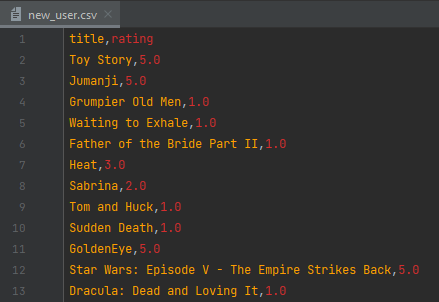
\includegraphics[scale=0.65]{images/new_user}
	\caption{Datos del nuevo usuario.}
	\label{new_user}
\end{figure}

Después de crear un nuevo dataframe con los datos del nuevo usuario, extraemos los títulos de las películas del conjunto de datos que el nuevo usuario haya visto, los guardamos en la variable \textit{titles}, y los unimos a los datos del nuevo usuario almacenados en el dataframe \textit{user\_df}. En este punto para ahorrar un poco de espacio en memoria, aprovechamos a eliminar la columna \textit{year} de \textit{user\_df}, ya que no se utilizará más adelante en el sistema de recomendación.

\begin{lstlisting}[language=python, basicstyle=\small]
titles = movies_df[movies_df['title'].isin(user_df['title'].tolist())]
user_df = pd.merge(titles, user_df)
user_df = user_df.drop('year', 1)
\end{lstlisting}

Así queda organizado el contenido en \textit{user\_df}:

\begin{table}[H]
	\centering
	\begin{tabular}{clc}
		\toprule
		movieId &                  title &  rating \\
		\midrule
		1 &                    Toy Story &     5.0 \\
		2 &                      Jumanji &     5.0 \\
		3 &             Grumpier Old Men &     1.0 \\
		4 &            Waiting to Exhale &     1.0 \\
		5 &  Father of the Bride Part II &     1.0 \\
		6 &                         Heat &     3.0 \\
		7 &                      Sabrina &     2.0 \\
		915 &                      Sabrina &     2.0 \\
		8 &                 Tom and Huck &     1.0 \\
		9 &                 Sudden Death &     1.0 \\
		\bottomrule
	\end{tabular}
	\caption{Contenido del dataframe \textit{user\_df}.}
	\label{user_df}
\end{table}

Observando la Tabla~\ref{user_df}, vemos que cada fila del dataframe \textit{user\_df} contiene un identificador de película, el título de la película y la valoración de esta realizada por el nuevo usuario. 

Siguiendo con la estrategia y una vez añadidos los títulos de las películas a los datos del nuevo usuario, podemos obtener todos los usuarios que hayan visto las mismas películas, que además agruparemos por su identificador de usuario (userId) con el método \textit{groupby}. En la Tabla~\ref{user_525}, se observan todas las películas valoradas por uno de los usuarios, concretamente las películas valoradas por el usuario 525.

\begin{lstlisting}[language=python, basicstyle=\small]
movies = ratings_df[ratings_df['movieId'].isin(user_df['movieId'].tolist())]
users = movies.groupby(['userId'])
\end{lstlisting}

\begin{table}[H]
	\centering
	\begin{tabular}{ccc}
		\toprule
		userId &  movieId &  rating \\
		\midrule
		525 &        1 &     4.0 \\
		525 &        2 &     3.5 \\
		525 &       34 &     3.0 \\
		525 &       39 &     4.5 \\
		525 &       48 &     3.0 \\
		525 &       62 &     3.5 \\
		525 &      107 &     3.5 \\
		525 &      150 &     4.0 \\
		525 &      223 &     3.5 \\
		525 &      377 &     3.5 \\
		525 &      480 &     4.0 \\
		525 &      595 &     3.5 \\
		525 &      915 &     3.5 \\
		525 &     1196 &     4.5 \\
		\bottomrule
	\end{tabular}
	\caption{Películas que ha visto y valorado el usuario 525.}
	\label{user_525}
\end{table}

Vemos que en total el usuario 525 ha valorado 14 películas, 12 de las cuales no han sido valoradas por el nuevo usuario (ver Tabla~\ref{user_df}). Este hecho podría entorpecer la predicción de las recomendaciones, así que, para una mejor predicción, ordenaremos a los usuarios de tal forma que los que compartan la mayor cantidad de películas tengan más prioridad (usuarios comunes).

\begin{lstlisting}[language=python, basicstyle=\small]
common_users = sorted(users, key=lambda x: len(x[1]), reverse=True)
\end{lstlisting}

\subsection{Coeficiente de Correlación Pearson}\label{correlacion_pearson}

Una vez encontrados los usuarios más comunes del conjunto de datos, ya podemos medir la similitud entre ellos para predecir las recomendaciones. El sistema de recomendación buscará correlaciones entre patrones de valoración sobre las películas que han valorado los usuarios y viendo cómo los usuarios se relacionan entre sí. Es decir, el sistema buscará las similitudes entre las valoraciones de las películas del nuevo usuario con el resto de usuarios para encontrar aquellos que se parecen más a este (usuarios similares). Para ello usaremos el \href{https://es.wikipedia.org/wiki/Coeficiente_de_correlaci\%C3\%B3n_de_Pearson}{coeficiente de correlación Pearson}. La fórmula para calcular el coeficiente de correlación Pearson sobre un estadístico muestral (ver Definición~\ref{estadístico_muestral}) se muestra a continuación:

\begin{equation}\label{formula}
	\large r = \frac{\sum_{1}^{n} \; (x_{i} - \bar{x}) (y_{i} - \bar{y})}{\sqrt{\sum_{1}^{n}(x_{i} - \bar{x})^2} \; \sqrt{\sum_{1}^{n}(y_{i} - \bar{y})^2}}
\end{equation}

Los valores dados por la fórmula (\ref{formula}) pueden variar entre [-1,1].

\begin{itemize}
	\item Si $r=1$ (correlación positiva perfecta), entonces las valoraciones estarán perfectamente correlacionadas. Los usuarios tendrán los mismos intereses.
	\item Si $0<r<1$, entonces existe una correlación positiva. Los usuarios tendrán intereses parecidos.
	\item Si $-1<r<0$, entonces existe una correlación negativa. Los usuarios tendrán pocos intereses parecidos.
	\item Si $r=-1$ (correlación negativa perfecta), entonces las valoraciones estarán inversamente correlacionadas. Los usuarios no tendrán los mismos intereses.
\end{itemize}

Se ha decidido usar el coeficiente de correlación Pearson como medida de similitud por una de sus propiedades. Esta propiedad nos dice que, si se multiplican todos los elementos por una constante distinta a cero o si se agrega cualquier constante a todos los elementos del coeficiente, este no cambiará con la escala. Por ejemplo, si tenemos dos vectores $X$ e $Y$, entonces $pearson(X,Y) = pearson(X,2\cdot Y+3)$. Esta es una propiedad muy importante en los sistemas de recomendación porqué si dos usuarios valoran dos elementos de manera completamente diferente, pero son usuarios muy parecidos (con intereses similares) contaríamos con valoraciones muy parecidas en escalas variadas y esto crearía grandes problemas en la predicción de las recomendaciones. El coeficiente de correlación Pearson es una de las medidas de similitud más utilizadas en un sistema de recomendación cuando hay variaciones entre magnitudes y escala en las valoraciones, aunque pudiéramos obtener valores altos de correlación si existen pocos usuarios con valoraciones en común.

\begin{definition}\label{estadístico_muestral}
En estadística un estadístico muestral es una medida cuantitativa, derivada de un conjunto de datos de una muestra, con el objetivo de estimar o inferir características de una población o modelo estadístico.
\end{definition}

A continuación, mostramos el código para calcular las similitudes entre los usuarios que se basa en los coeficientes de correlación Pearson. Los coeficientes los almacenaremos en un diccionario que llamaremos \textit{pearsonCorrelationDict}, donde las claves serán los identificadores de los usuarios y los valores de cada clave serán los coeficientes. Elegimos un subconjunto de usuarios (\textit{usersSubset}) para realizar menos iteraciones y no añadir demasiado sobrecoste computacional. El subconjunto de usuarios está formado por 100 usuarios.

\begin{lstlisting}[language=python, basicstyle=\small]
usersSubset = common_users[0:100]	
pearsonCorrelationDict = {}

for id, group in usersSubset:
	# The current user and the new user are ordered in the same way
	user = group.sort_values(by='movieId')
	movies = user_df.sort_values(by='movieId')
	
	# Number of ratings for user
	nRatings = len(user)
	
	# Common ratings of the current user with the new user
	temp_df = movies[movies['movieId'].isin(user['movieId'].tolist())]
	tempRatingList = temp_df['rating'].tolist()
	
	# Ratings of the current user
	tempUserList = user['rating'].tolist()
	
	# Calculate the Pearson Correlation between the current user and new user
	Uxx = sum([i ** 2 for i in tempRatingList])-pow(sum(tempRatingList), 2) / float(nRatings)
	Uyy = sum([i ** 2 for i in tempUserList])-pow(sum(tempUserList), 2) / float(nRatings)
	Uxy = sum(i * j for i, j in zip(tempRatingList, tempUserList))-sum(tempRatingList) * sum(tempUserList) / float(nRatings)
	
	# If the denominator is nonzero, then we divide, otherwise the correlation is 0
	if Uxx != 0 and Uyy != 0:
		pearsonCorrelationDict[id] = Uxy / sqrt(Uxx * Uyy)
	else:
		pearsonCorrelationDict[id] = 0
\end{lstlisting}

Inicialmente en cada iteración, se ordenan los datos de cada usuario instanciado y los datos del nuevo usuario de la misma manera, para que los valores no se mezclen más adelante. Después se obtiene el número de valoraciones del usuario instanciado y se obtienen las valoraciones en común de este con el nuevo usuario, y todo se almacena en una lista temporal llamada \textit{tempRatingList}. Guardamos también en una lista temporal las valoraciones del usuario instanciado (\textit{tempUserList}). 

\newpage 

En definitiva, la finalidad de esta parte del código es calcular los coeficientes de correlación Pearson de cada usuario instanciado con el nuevo usuario basándonos en la fórmula (\ref{formula}), siempre comprobando que el dominador sea diferente a cero, sino el valor del coeficiente será 0. El contenido del diccionario \textit{pearsonCorrelationDict} después de realizar todas las iteraciones es el siguiente:

\begin{lstlisting}[language=bash, basicstyle=\small]
dict_items([(414, 0.1710335374313876), (599, 0.40123525382704545), (6, 0.20329349941761546), (474, 0.21044663004441924), (274, 0.3530769675354643), (68, 0.33059489678211385), (608, 0.3260682075724168), (182, -0.23109387695394956), (19, 0.3133595303614617), (307, -0.18843150346003273), (91, 0.31180055592445977), (314, -0.1855577860558229), (380, 0.45012727283065757), (84, 0.012277750762966397), (117, -0.06953551887224728), (480, 0.16458728710301657), (217, 0.3252127201443157), (483, -0.16673896789941262), (372, 0.05020839625891806), (470, 0.32705689114535186), (489, -0.025392998342644958), (600, 0.042693983860009506), (240, 0.05131981034870924), (337, 0.3214285714285713), (448, 0.3145474121592105), (559, 0.17567351114860863), (602, -0.01953661662911384), (603, -0.12466125165644129), (604, -0.11070047639148746), (226, -0.08878401871687391), (43, -0.4295675016629953), (57, 0.05739773181955021), (160, -0.23053561726821561), (181, -0.025450425803285343), (411, 0.4184472097595221), (492, 0.009531160645787254), (524, 0.554930806561758), (45, 0.38256520195621246), (58, 0.06698696164390111), (109, -0.08767933833518694), (288, 0.040138052643118996), (304, -0.05079155413724917), (438, 0.1689463508123878), (592, 0.06429719695335717), (597, -0.04354691441125118), (40, -0.046609537669447546), (64, 0.027500104500595552), (446, -0.29551933110701833), (501, -0.021239769762143604), (590, 0.1779059797601214), (191, -0.5019578060538685), (219, 0.48620274802831803), (284, -0.00550473542118167), (353, 0.20638197410277853), (386, -0.1111123018786146), (140, -0.08363570955493667), (357, -0.009026976808426818), (373, -0.13235807087846027), (42, -0.010032434901514608), (136, -0.1711753075974906), (177, 0.1690569419933152), (179, 0.09896799408051585), (249, 0.25782317138405986), (330, -0.0750008147037369), (368, 0.2405974233356921), (437, 0.04624821484746095), (477, 0.31049173032627525), (594, 0.008390572815346994), (18, 0.019351013185103308), (103, -0.003498129001342704), (112, 0.38778864063592566), (385, 0.5296480205051889), (387, 0.43198485996958375), (425, 0.09288282368076137), (541, 0.25728140367086977), (566, 0.0679837639353997), (584, 0.573224999318389), (32, -0.04999999999999922), (235, -0.30774536098405614), (266, 0.177355756021643), (391, -0.3687156994355351), (428, -0.24008629652200658), (458, 0.0843349010400103), (469, 0.10400998543792594), (555, -0.006953000128056482), (570, 0.2575275846563296), (580, 0.31742024784266926), (94, 0.5774257546144353), (144, -0.25560087159134015), (294, 0.4777456720827587), (318, -0.40396888282756127), (323, 0.2786429232355919), (381, 0.07479684684631624), (453, 0.0), (486, 0.3959797974644654), (534, 0.23281019568466926), (588, -0.16115829864721526), (606, -0.4177121530460993), (82, 0.3263157894736842), (121, -0.1532100435348196)])
\end{lstlisting}

Aunque hemos incluido los usuarios más comunes a la hora de calcular la similitud entre usuarios, vemos que la estimación no es muy realista, los valores de los coeficientes son bajos. Puede que el valor de iteraciones límite determinado en función de los datos disponibles y de su robustez no sea el adecuado. Esto puede deberse a que, para algunas películas, no haya suficientes usuarios que las hayan valorado. A pesar de esta estimación se sigue con la construcción del sistema de recomendación y guardamos el contenido del diccionario \textit{pearsonCorrelationDict}, para una mejor visualización, en un nuevo dataframe que llamaremos \textit{pearson\_df}. El nuevo dataframe tiene dos columnas, la columna \textit{similarityIndex} que contiene los coeficientes de correlación Pearson y la columna \textit{userId} que contiene los identificadores de los usuarios.

\begin{lstlisting}[language=python, basicstyle=\small]
pearson_df = pd.DataFrame.from_dict(pearsonCorrelationDict, orient='index')
pearson_df.columns = ['similarityIndex']
pearson_df['userId'] = pearson_df.index
pearson_df.index = range(len(pearson_df))
\end{lstlisting}

\newpage

Así queda organizado el contenido en \textit{pearson\_df}:

\begin{table}[H]
	\centering
	\begin{tabular}{cc}
		\toprule
		similarityIndex &  userId \\
		\midrule
		0.171034 &     414 \\
		0.401235 &     599 \\
		0.203293 &       6 \\
		0.210447 &     474 \\
		0.353077 &     274 \\
		0.330595 &      68 \\
		0.326068 &     608 \\
		-0.231094 &     182 \\
		0.313360 &      19 \\
		-0.188432 &     307 \\
		\bottomrule
	\end{tabular}
	\caption{Contenido del dataframe \textit{pearson\_df}.}
\label{pearson_df}
\end{table}


\subsection{Predicción y Resultado}\label{resultados}

Como tenemos ordenado el conjunto de datos de tal forma que los usuarios que comparten la mayor cantidad de películas tienen más prioridad, podemos realizar una selección de vecindario. La selección de vecindario o la selección de los $K$ vecinos más cercanos, es la aproximación más común para seleccionar los $K$ usuarios más similares de un nuevo usuario. $K$ es el número de vecinos que vamos a seleccionar, en teoría cuantos más vecinos seleccionemos para nuestro vecindario mejores recomendaciones realizará el sistema de recomendación. Porqué aplicando una selección de vecindario conseguiremos penalizar aquellas situaciones donde el cálculo de la similitud entre los usuarios haya obtenido pocas valoraciones en común, como parece ser que hemos observado en la sección anterior. En este caso, seleccionamos el valor de $K$ igual a 50. Los 50 usuarios seleccionados son ordenados por sus coeficientes de forma ascendente, así en las primeras posiciones tendremos los usuarios más parecidos al nuevo usuario.

\begin{lstlisting}[language=python, basicstyle=\small]
topUsers = pearson_df.sort_values(by='similarityIndex', ascending=False)[0:50]
\end{lstlisting}

Veamos los primeros 10 usuarios más parecidos al nuevo usuario, que en este caso como yo he valorado las películas según mi criterio, son los primeros 10 usuarios más parecidos a mí.

\begin{table}[h]
	\centering
	\begin{tabular}{cc}
		\toprule
		similarityIndex &  userId \\
		\midrule
		0.577426 &      94 \\
		0.573225 &     584 \\
		0.554931 &     524 \\
		0.529648 &     385 \\
		0.486203 &     219 \\
		0.477746 &     294 \\
		0.450127 &     380 \\
		0.431985 &     387 \\
		0.418447 &     411 \\
		0.401235 &     599 \\
		\bottomrule
	\end{tabular}
	\caption{Los 50 usuarios más similares al nuevo usuario.}
	\label{top_50}
\end{table}

Parece ser que mis intereses no son muy similares a los de los otros usuarios que forman el conjunto de datos. Los coeficientes de correlación Pearson que podemos observar en la Tabla~\ref{top_50} no son muy altos. Por ejemplo, el valor de similitud con el usuario que más se parece a mí, el usuario 94, es igual a 0.577426. Aun así, vamos a calcular las recomendaciones. Aún así, tomaremos la media ponderada de las valoraciones de las películas utilizando los coeficientes de la correlación Pearson. Se ha elegido la media ponderada como medida de predicción porqué se considera fácil de calcular y suele funcionar bastante bien, aunque no tiene en cuenta el sesgo en las valoraciones de los usuarios si tienden a valorar alto o bajo. 

La media ponderada se calcula aplicando la siguiente fórmula:

\begin{equation}\label{media_ponderada}
	\large \hat{r}_{u,i} = \frac{1}{\sum_{a\in K}sim(u,a)} \sum_{a\in K }sim(u,a) r_{a,i}
\end{equation}

A fin de calcular la media ponderada, primero debemos unir las valoraciones de todas las películas del dataframe \textit{ratings\_df} con los usuarios más similares al nuevo usuario (\textit{topUsers}). Guardamos el resultado de la unión en un nuevo dataframe que llamamos \textit{topUsersRating}. A la hora de realizar esta unión usamos la función \textit{merge} de la librería pandas, que nos permite realizar la unión de los dos dataframes (\textit{ratings\_df} y \textit{topUsersRating}) sobre las columnas \textit{userId}, considerando solo las filas con etiquetas comunes (\textit{inner}). 

\begin{lstlisting}[language=python, basicstyle=\small]
topUsersRating = topUsers.merge(ratings_df, left_on='userId', right_on='userId', 
	how='inner')
\end{lstlisting}

Vemos como queda organizado el contenido de \textit{topUsersRating}:

\begin{table}[H]
	\centering
	\begin{tabular}{cccc}
		\toprule
		similarityIndex &  userId &  movieId &  rating \\
		\midrule
		0.577426 &      94 &        2 &     4.0 \\
		0.577426 &      94 &       10 &     3.0 \\
		0.577426 &      94 &       11 &     3.0 \\
		0.577426 &      94 &       17 &     1.0 \\
		0.577426 &      94 &       19 &     2.0 \\
		0.577426 &      94 &       21 &     3.0 \\
		0.577426 &      94 &       32 &     5.0 \\
		0.577426 &      94 &       34 &     4.0 \\
		0.577426 &      94 &       39 &     1.0 \\
		0.577426 &      94 &       44 &     1.0 \\
		\bottomrule
	\end{tabular}
	\caption{Unión de los dataframes \textit{ratings\_df} y \textit{topUsersRating}.}
	\label{ratings_similares}
\end{table}

A continuación, calculamos la media ponderada aplicando la fórmula (\ref{media_ponderada}). El cálculo se realiza sencillamente multiplicando las columnas \textit{similarityIndex} y \textit{rating} del dataframe \textit{topUsersRating}; y guardando el resultado en una nueva columna (\textit{weightedRating}). Ver la Tabla~\ref{weightedRating}.

\begin{lstlisting}[language=python, basicstyle=\small]
topUsersRating['weightedRating'] = topUsersRating['similarityIndex'] * topUsersRating['rating']
\end{lstlisting} 

Después se suman los valores de las columnas \textit{similarityIndex} y \textit{weightedRating}, y se agrupan por la columna \textit{movieId}. Por último, separamos el resultado en dos columnas: la columna \textit{sum\_similarityIndex} que contiene las sumas de los coeficientes de correlación Pearson, y la columna \textit{sum\_weightedRating} que contiene las sumas de las valoraciones de los usuarios por los coeficientes. Ver la Tabla~\ref{sums}.

\begin{lstlisting}[language=python, basicstyle=\small]
tempTopUsersRating = topUsersRating.groupby('movieId').sum()[['similarityIndex', 'weightedRating']]
tempTopUsersRating.columns = ['sum_similarityIndex', 'sum_weightedRating']
\end{lstlisting} 

\begin{table}[H]
	\centering
	\begin{tabular}{ccccc}
		\toprule
		similarityIndex &  userId &  movieId &  rating &  weightedRating \\
		\midrule
		0.577426 &      94 &        2 &     4.0 &        2.309703 \\
		0.577426 &      94 &       10 &     3.0 &        1.732277 \\
		0.577426 &      94 &       11 &     3.0 &        1.732277 \\
		0.577426 &      94 &       17 &     1.0 &        0.577426 \\
		0.577426 &      94 &       19 &     2.0 &        1.154852 \\
		0.577426 &      94 &       21 &     3.0 &        1.732277 \\
		0.577426 &      94 &       32 &     5.0 &        2.887129 \\
		0.577426 &      94 &       34 &     4.0 &        2.309703 \\
		0.577426 &      94 &       39 &     1.0 &        0.577426 \\
		0.577426 &      94 &       44 &     1.0 &        0.577426 \\
		\bottomrule
	\end{tabular}
	\caption{Multiplicación de las columnas \textit{similarityIndex} y \textit{rating}.}
	\label{weightedRating}
\end{table}

\begin{table}[H]
	\centering
	\begin{tabular}{cc}
		\toprule
		sum\_similarityIndex &  sum\_weightedRating \\
		\midrule
		11.302189 &           43.880774 \\
		9.326976 &           30.408888 \\
		4.882914 &           12.700033 \\
		0.621741 &            1.446775 \\
		2.796576 &            8.189528 \\
		8.893940 &           34.706954 \\
		3.739738 &           10.699062 \\
		0.727404 &            2.182212 \\
		1.353227 &            4.100684 \\
		11.269351 &           40.952455 \\
		\bottomrule
	\end{tabular}
	\caption{Las columnas \textit{sum\_weightedRating} y \textit{sum\_weightedRating}.}
	\label{sums}
\end{table}

Por último, se divide el contenido de las columnas \textit{sum\_weightedRating} y \textit{sum\_weightedRating}. Como resultado de ello obtenemos los valores de la media ponderada que se almacenan en la columna \textit{weighted\_average\_score} de un nuevo dataframe que llamamos \textit{recommendation\_df}. Junto con los valores de la media ponderada también se almacenan los identificadores de las películas (movieId).

\begin{lstlisting}[language=python, basicstyle=\small]
recommendation_df = pd.DataFrame()
recommendation_df['weighted_average_score'] = tempTopUsersRating['sum_weightedRating']/tempTopUsersRating['sum_similarityIndex']
recommendation_df['movieId'] = tempTopUsersRating.index
\end{lstlisting}

Vemos como queda organizado el contenido de \textit{recommendation\_df}:

\begin{table}[H]
	\centering
	\begin{tabular}{cc}
		\toprule
		weighted\_average\_score &  movieId \\
		\midrule
		3.882502 &        1 \\
		3.260316 &        2 \\
		2.600913 &        3 \\
		2.326975 &        4 \\
		2.928412 &        5 \\
		3.902315 &        6 \\
		2.860912 &        7 \\
		\bottomrule
	\end{tabular}
	\caption{Media ponderada por película.}
	\label{promedio_ponderado_resultado}
\end{table}

Una vez calculados los valores de la media ponderada, se ordenan de forma ascendente para mostrar los primeros 10 valores más altos, o que es lo mismo, las primeras 10 películas que recomienda el sistema de recomendación al nuevo usuario. Podemos observar estas recomendaciones en la Tabla~\ref{recomendaciones_finales}.

\begin{lstlisting}[language=python, basicstyle=\small]
recommendation_df = recommendation_df.sort_values(by='weighted_average_score', ascending=False)
recommendation_df = movies_df.loc[movies_df['movieId'].isin(recommendation_df.head(10)['movieId'].tolist())]
\end{lstlisting}

\begin{table}[H]
	\centering
	\begin{tabular}{clc}
		\toprule
		movieId &                         title &  year \\
		\midrule
		2295 &                   Impostors, The &  1998 \\
		7121 &                       Adam's Rib &  1949 \\
		74754 &                        Room, The &  2003 \\
		82744 &                           Faster &  2010 \\
		95149 &  Superman/Batman: Public Enemies &  2009 \\
		102084 &             Justice League: Doom &  2012 \\
		108795 &                     Wonder Woman &  2009 \\
		147376 &    Doctor Who: A Christmas Carol &  2010 \\
		172875 &                A Detective Story &  2003 \\
		173145 &   War for the Planet of the Apes &  2017 \\
		\bottomrule
	\end{tabular}
	\caption{Las 10 mejores recomendaciones.}
	\label{recomendaciones_finales}
\end{table}

A pesar de una estimación inicial que parecía poco realista y que podríamos llegar a intuir que el sistema podría no dar una buena recomendación a causa de que mis intereses no se parecían mucho a los de los otros usuarios, el sistema de recomendación des de mi punto de vista me ha dado una buena recomendación. Me gustan mucho las películas de superhéroes i de ciencia ficción. También me gustan bastante las películas de temática policíaca. Aunque el sistema de recomendación ha patinado un poco al recomendarme la película "Room, The", no le vería nunca.

\section{Conclusiones}

En este documento se ha descrito una sencilla implementación en Python de un sistema de recomendación de filtrado colaborativo basado en usuarios, con el fin de recomendar películas a un nuevo usuario según sus intereses. Paso a paso se ha ido describiendo el desarrollo del sistema de recomendación, hasta obtener las recomendaciones que han sido buenas. Llegando a la conclusión que, aunque seguramente el sistema de recomendación se podría mejorar adoptando un enfoque híbrido y así aprovechar las ventajas de los sistemas colaborativos y los no colaborativos, contar con sistemas de recomendación que ayuden a los usuarios a buscar información y tomar decisiones en este entorno es un tema muy útil y de crucial importancia.

Quiero destacar como valoración personal, que he elegido hacer un ejercicio práctico para llevar a cabo la teoría aprendida durante el aprendizaje teórico. Siempre me parece muy interesante llevar a la práctica conocimiento nuevo para ver su utilidad. He escogido un sistema de recomendación de filtrado colaborativo basado en usuarios, porque me ha parecido el adecuado y más sencillo de llevar a la práctica. 

Sé que existen muchísimos sistemas de recomendación ya implementados, pero me pareció muy interesante desarrollar un sistema de recomendación propio, muy básico y simple de entender. Además, nunca había intentado implementar un sistema de recomendación en ningún tipo de lenguaje de programación. Decidí que fuera en Python, ya que es el lenguaje que uso más a diario y es uno de los lenguajes de programación más utilizados en el mundo, además uno de los mayores aliados para la Ciencia de Datos. 

Se podrían consideran muchas mejoras en el sistema de recomendación desarrollado en esta práctica, seguramente las primeras que realizaría en un futuro con más tiempo, serían la automatización de la creación de un nuevo usuario y añadir la modularización.

\renewcommand{\refname}{Bibliografía}
\bibliographystyle{unsrt}
\bibliography{biblio}
	
\end{document}
